\documentclass[11pt]{article}
\usepackage[letterpaper, margin=1in]{geometry}
% \usepackage[skip=\baselineskip, tocskip=0pt]{parskip}
\usepackage{amsmath, amsfonts, amssymb, amsthm, mathtools}
\usepackage{stmaryrd}
\usepackage{fontspec}
\let\latextextsubscript\textsubscript
\AtBeginDocument{
  \let\textsubscript\latextextsubscript
  \newcommand{\sub}[1]{\textsubscript{#1}}
  \newcommand{\gap}[1]{\rule{1em}{0.4pt}\textsubscript{#1}}
}
\let\latextextsuperscript\textsuperscript
\AtBeginDocument{
  \let\textsuperscript\latextextsuperscript
}
\usepackage[largesc]{newpxtext}
\usepackage[vvarbb]{newpxmath}
\usepackage[threshold=1]{csquotes}
% \usepackage{markdown}

\usepackage{pifont}
% \usepackage{txfonts}
\let\eachwordone=\rmfamily
\let\eachwordtwo=\rmfamily
\let\eachwordthree=\rmfamily
\let\rm=\relax
\usepackage[linguex]{expex-glossonly}
\lingset{everygla={\itshape}}
\renewcommand{\firstrefdash}{}
% \usepackage{hyperref}
% \usepackage{cleveref}
% \crefname{ExNo}{}{}
% \crefname{SubExNo}{}{}
% \renewcommand{\theExNo}{\arabic{ExNo}}
% \renewcommand{\theSubExNo}{\theExNo\alph{SubExNo}}
% \creflabelformat{SubExNo}{(#2#1#3)}
% \creflabelformat{ExNo}{(#2#1#3)}
% \crefrangelabelformat{SubExNo}{(#3#1#4--#5\crefstripprefix{#1}{#2}#6)}
% \crefrangelabelformat{ExNo}{(#3#1#4)--(#5#2#6)}
% \usepackage{enumitem}
% \usepackage[normalem]{ulem}
% \usepackage{xcolor}
%
% \usepackage{paracol}
% \usepackage{eqparbox}
% \setlength{\columnseprule}{.4pt}
% \globalcounter{ExNo}
\setlength{\parskip}{1ex}
\setlength{\parindent}{0pt}
% \setlist[1]{left=0pt}
% \renewcommand\thesection{\Roman{section}.}
% \renewcommand\thesubsection{\arabic{subsection}.}
% \renewcommand\thesubsubsection{\Alph{subsubsection}}

% \usepackage[
%   backend=biber,
%   natbib=true,
%   style=unified,
%   maxcitenames=3,
%   maxbibnames=99
% ]{biblatex}
% \addbibresource{../Distributivity.bib}
\AtBeginDocument{
  % \setlength{\Extopsep}{0\baselineskip}
  % \setlength{\Exredux}{0\baselineskip}
  \settowidth{\Exlabelwidth}{(00)}
  % \setlength{\Exlabelwidth}{.7\Exlabelwidth}
  % \setlength{\Exlabelsep}{.7\Exlabelsep}
  % \setlength{\SubExleftmargin}{\SubExleftmargin}
  % \setlength{\SubSubExleftmargin}{\SubSubExleftmargin}
}

\newcommand{\A}{\(\overline{\text{A}}\)}
% \usepackage{tikz}
\usepackage[linguistics]{forest}
% \usetikzlibrary{positioning}
% \usetikzlibrary{arrows.meta}
% \usetikzlibrary{tikzmark}
% \usepackage{tikz-cd}
% \tikzcdset{
%   arrow style=math font,
%   % diagrams={>={Straight Barb[scale=0.8]}}
% }
%
% \tikzset{every label/.style={font=\footnotesize}}
%
% \forestset{
%   default preamble={
%     for tree={
%       inner sep=0pt,
%       % draw,
%     }
%   },
%   great empty nodes/.style={
%     for tree={
%       calign=fixed edge angles,
%       calign primary angle=-60,
%       calign secondary angle=60, 
%     l=7mm},
%     delay={
%       where content={}{
%         shape=coordinate,
%     for current and siblings={anchor=north}}{}}
%   },
%   downroof/.style={
%     for children={
%       if n=1{
%         edge path'={
%           (.parent first) -- (!u.parent anchor) -- (!ul.parent last) -- cycle
%         }
%       }{no edge}
%     }
%   }
% }
% \usepackage{tabularx}
% \usepackage{booktabs}
% \renewcommand\tabularxcolumn[1]{m{#1}}% for vertical centering text in X column

\usepackage{langsci-avm}
\AtBeginDocument{% to do this after unicode-math has done its work
  \renewcommand{\setminus}{\mathbin{\backslash}}%
}
\title{(Copy) Raising in LFG/HPSG}
\author{Haoming Li, Taieba Tawakoli, Giovanni Roversi}
%
% \DeclareMathOperator{\atom}{\textsc{Atom}}
% \DeclareMathOperator{\alt}{\textsc{Alt}}
% \DeclareMathOperator{\xh}{\textsc{Exh}}
% \newcommand{\exh}{\ensuremath{\xh}}
% \newcommand{\Exh}{\ensuremath{\mathcal{E}\mathit{xh}}}
% \newcommand{\Pex}{\ensuremath{\mathcal{P}\mathit{ex}}}
% \DeclareMathOperator{\prt}{Part}
% \DeclareMathOperator{\dom}{dom}
% \newcommand{\dexh}{\ensuremath{D_{\textnormal{exh}}}}
% \newcommand{\dpart}{\ensuremath{D_{\textnormal{part}}}}
\begin{document}
\maketitle

\avmsetup{values=\normalfont,switch=*}
\section{HPSG – Kay (2021): ``Copy raising as a lexical rule''}
\label{sec:sbcg_a_dialect_of_hpsg}
% {\color{red}
% \begin{itemize}
% \item Empirical observation: \begin{itemize}
%     \item A) Every CR verb has a corresponding general perception verb
%     \item B) As-if clause is a constituent (3) \begin{itemize}
%         \item ``Like'' has its own lexical entry, marking the embedded clause as an ``as-if'' object
%         \end{itemize}
%     \end{itemize}

% \item Lexical rule: perception verb $\leftarrow$ CR verb \begin{itemize}
%     \item Talk about XARG: sort of a version of SPR that ``passes up'' the tree instead of disappearing, making information available between the embedded and matrix clause
%     \end{itemize}

% \item Full analysis in big tree
% \end{itemize}}

\begin{itemize}
  \item (Technically a paper employing Sign-Based Construction Grammar (SBCG), a dialect of HPSG; you can find a discussion of SBCG in the last chapter of the \textit{Syntactic Theory} textbook)

  \item Baseline example of Copy Raising (CR):
\end{itemize}
\ex. Trump seems like he disappeared.

\begin{itemize}
  \item Two main empirical observations they're trying to capture: \begin{itemize}
      \item Every CR verb has a corresponding ``general perception'' verb (\textit{look, seem, appear, sound})
      \item The \textit{like\slash as if \slash as though} clause behaves as a constituent, an obligatory complement of the matrix verb
    \end{itemize}



  \item Core idea of the analysis: \textbf{CR is derived with a lexical rule}, that takes in a general perception verb and outputs a CR verb.

  \item The following lexical entry for \emph{like} captures the idea that \emph{like} forms a constituent with the clause
\end{itemize}
\ex. 
\avm{
  [
    form & <\type{like}> \\
    syn & [
      cat & [
        \type{adverb} \\
        xarg & \type{none} \\
        select & [
          \type*{verb} \\
          syn & [
            cat & [
              vform & \type{fin} \\
              xarg & NP \\
              inv & \(-\)
            ] \\
            val & < & >
          ] \\
          sem & [
            ltop & \(l\) \\
            index & \(e\)
          ]
        ]
      ] \\
      val & < & > \\
      mrkg & \type{asif}
    ] \\
    sem & [
      frames & < *\type{as-if}\((e', l)\)* > \\
      index & \(e'\)
    ]
  ]
}

\begin{itemize}
  \item Some explanations of features introduced in SBCG:
    \begin{itemize}
      \item  The \textsc{xarg} feature talks about the external argument, like \textsc{spr} in HPSG; however, \textsc{xarg} is different from \textsc{spr} in that it is visible to outside structure even after the merger with the external argument.
      \item The \textsc{val(ence)} feature is like \textsc{arg-st} in HPSG, but with the difference that \textsc{arg-st} can contain `extracted' or unexpressed arguments, \textsc{val} does not.
      \item In addition to specifying that \emph{like} forms a constituent with the clause, it also imposes 
        \begin{itemize}
          \item The finiteness of the clause (\avm{[vform & \type{fin}]})
          \item A pronoun in the external-argument position of the clause (\avm{[xarg & NP]})
          \item That the resulting constituent is marked as \emph{asif} (\avm{[mrkg & \type{asif}]})
        \end{itemize}
    \end{itemize}
  \item The lexical rule for CR verbs should achieve the following effect minimally, as stated in the constraint:
\end{itemize}
\ex. \avm{
  [ mtr & [val <NP\(_i\), S[mrkg \type{asif}, xarg NP[\type{pron}]\(_i\)]>] ]
}

\begin{itemize}
  \item This says that the subject of the copy-raising predicate must be co-indexed with a pronoun in the external argument position of the complement of the predicate, and the predicate must be marked as \avm{\type{asif}}.
  \item The following is the fully spelled-out lexical rule for deriving CR verbs from general perception verbs:
\end{itemize}
\ex. \avm{
  [
    mtr & \(X\)! [
      syn & [
        cat & [xarg \(Z\):NP\(_i\)] \\
        val & <\(Z\), [
          syn & [
            cat & [
              vform & \type{fin} \\
              xarg & NP[\type{pron}]\(_i\)
            ] \\
            val & < & > \\
            mrkg & \type{asif}
          ] \\
          sem & [
            ltop & \(l\)
          ]
        ]> 
      ] \\
      sem & [
        frames & <*\type{seeming-fr}\((e)\)*, *\type{human-fr}\((j)\)*, \(l\)>\\
        index & \(e\)
      ]
    ] \\
    dtrs & <\(X\):[
      \type{verb} \\
      sem & [ frames & < *\type{gen-perception-fr}\((e)\)* > ]
    ]>
  ]
}

\begin{itemize}
  \item Some explanations:
    \begin{itemize}
      \item Basically, \textsc{mtr} (\textsc{mother}) tells us the output of lexical rules, while \textsc{dtrs} (\textsc{daughters}) tells us the input(s) of lexical rules; thus this rule tells that we can make a CR verb out of any general perception verb.
      \item  The notation \avm{\(X\)! [A]} and \avm{\(X\):[B]} indicate that \avm{[A]} and \avm{[B]} are identical in all respects in which they are not shown to differ.
      \item  Syntactically, copy-raising predicates requires a finite complement clause that has an external argument which is a pronoun; its own external argument must be co-indexed with the pronoun; note the index \(i\) on the value of \textsc{xarg} of both \(X\) and its complement.
      \item Semantically, copy-raising predicates involve a seeming event \(e\), and an experiencer \(j\).
    \end{itemize}
  \item Now, a fully represented analysis for the following example is provided:
\end{itemize}
\ex. Trump looks like he disappeared.

\begin{itemize}
  \item The tree for \Last:
\end{itemize}
\ex. \scalebox{0.8}{\begin{forest}
    for tree={fit=tight}
    [\avm{[
          form & <\type{trump,looks,like,he,disappeared}> \\
          syn & [
            cat & [
              \type{verb} \\
              xarg & NP\(_i\) 
            ] \\
            val & < & > \\
            mrkg & \type{unmrk}
          ] \\
          sem & [
            frames & <*\(l_1\), \(l_2\), \(l_3\), \(l_4\)*>
          ]
      ]}
      [\avm{[
            form & <\type{trump}> \\
            syn & \type{pn-word} \\
            sem & [
              frames & <*\(l_4\): \type{name-fr}\((i,\)\type{trump}\()\)*> \\
              index & \(i\)
            ]
      ]}]
      [\avm{[
            form & <\type{looks,like,he,disappeared}> \\
            syn & [
              cat & \type{verb} \\
              val & <\2> \\
              mrkg & \type{unmrk}
            ] \\
            sem & [
              frames & <*\(l_1\), \(l_2\), \(l_3\)*>
            ] \\
            % cntxt & \3
        ]}
        [\avm{[
              form & <\type{looks}> \\
              syn & [
                cat & [
                  \type{verb} \\
                  xarg & \2 NP\(_i\)
                ] \\
                val & <\2, \4 S [
                  mrkg & \type{asif} \\
                  xarg & NP[\type{pron}]\(_i\)
                ]> \\
                mkrg & \type{unmrk}
              ] \\
              sem & [
                frames & <
                *\(l_3\): \type{generic-fr}\((j)\)*, & \\
                *\(l_3\): \type{human-fr}\((j)\)*, & \\
                *\(l_3\): \type{seeming-fr}\((e'', j, l_2)\)*, &\\
                *\(l_3\): \type{present-fr}\((e'')\)* & 
                > \\
                index & \(e''\)
              ]
        ]}]
        [\avm{\4[
              form & <\type{like,he,disappeared}> \\
              syn & [
                cat & [
                  \type{verb} \\
                  xarg & NP[\type{pron}]\(_i\)
                ] \\
                val & < & > \\
                mrkg & \type{asif}
              ] \\
              sem & [
                ltop & \(l_2\) \\
                frames & <*\(l_2\)*, *\(l_1\)*>
              ] \\
              % cntxt & \3
            ]
          }
          [\avm{[
                form & <\type{like}> \\
                syn & [
                  cat & [select & \1] \\
                  mrkg & \type{asif}
                ] \\
                sem & [
                  frames & <*\(l_2\): \type{as-if}\((e', l_1)\)*> \\
                  index \(e'\)
                ]
          ]}]
          [\avm{\1[
                form & <\type{he,disappeared}> \\
                syn & [
                  cat & [
                    \type{verb} \\
                    xarg & NP[\type{pron}]\(_i\)
                  ] \\
                  val & < & > \\
                  mrkg & \type{unmrk}
                ] \\
                sem & [
                  ltop & \(l_1\) \\
                  frames & <
                  *\(l_1\): \type{disappear-fr}\((e, i)\)*, & \\
                  *\(l_2\): \type{past-fr}\((e)\)* &
                  > \\
                  index & \(e\)
                ]
          ]}]
        ]
      ]
    ]
\end{forest}}




\section{LFG – Camilleri (2017): ``On Raising And Copy Raising In Maltese''}
\label{sec:lfg}

\subsection{Regular raising}

\begin{itemize}
  \item Core part: \textbf{structure sharing} between matrix subject and an open position of the complement (clause), \textsc{xcomp} \begin{itemize}
      \item Fairly textbook LFG treatment of raising
    \end{itemize}
\end{itemize}

\ex. \begingl
\gla It-tfal ji-dhr-u (li) sejr-in tajjeb //
\glb \textsc{def}-children 3-appear.\textsc{impv-pl} \textsc{comp} go.\textsc{act.ptcp-pl} good //
\glft `The children seem to be doing well' //
\endgl

\begin{itemize}
  \item Relevant parts in the lexical entry for the raising predicate \emph{deher}:
\end{itemize}

\ex.  \begin{align*}
  (\uparrow \textsc{pred}) = \left\langle \textsc{xcomp} \right\rangle \textsc{subj} \\
  ((\uparrow \textsc{xcomp compform} = \textsc{li})) \\
  (\uparrow \textsc{subj}) = (\uparrow \textsc{xcomp subj}) \\
\end{align*}

\begin{itemize}
  \item In prose: \begin{itemize}
      \item My mother's \textsc{pred} value is $\left\langle \textsc{xcomp} \right\rangle \textsc{subj}$
      \item This \textsc{xcomp} is introduced by a complementizer of the form \textit{li}
      \item My mother's subject is the same as the \textsc{xcomp}'s subject
    \end{itemize}

  \item The \(f\)-structure for (7):
\end{itemize}
\ex. \avm{[
    pred & `\emph{jidhru} <xcomp>\textsc{subj}' \\
    subj & \1 [
      pred & `\emph{itfal}' \\
      pers & 3 \\
      num & \textsc{pl} \\
      def & \(+\)
    ] \\
    xcomp & [
      pred & `\emph{sejrin} <subj>' \\
      subj & \1 \\
      adj & \{[
          pred & `\emph{tajjeb}'
      ]\}
    ]
]}



\subsection{Copy Raising}

\begin{itemize}
  \item Baseline example: the matrix subject is coindexed with a pronominal argument (here, the object clitic) in the embedded clause.

  \item The item \textit{bħal} `like' is essentially doing the predicate job.
\end{itemize}
\ex. \begingl
\gla \textbf{it-tifla} bħal ta-w-\textbf{ha} xebgħa //
\glb \textbf{\textsc{def}-girl} like give.\textsc{pfv.3-pl-\textbf{3sgf.acc}} smacking //
\glft `The girl's as though they gave her a smacking' //
\endgl

\begin{itemize}
  \item Regular raising verbs and CR verbs have the same lexical entry: structure sharing with \textsc{xcomp}

  \item Therefore, CR has a slightly more involved derivation, with an ``extra layer'': \begin{itemize}
      \item Regular raising: the structure sharing is between matrix subject and embedded subject
      \item CR: structure sharing between matrix subject \emph{and subject of `like'}
      \item The actual coindexation between the matrix subject and the corresponding pronominal argument in the embedded clause is done \emph{semantically} (therefore, not represented in the f-structure)
      \item The semantic mechanism is conceptually similar to null operator movement\slash lambda abstraction: it opens up a slot (semantically) in the embedded clause, turning the clause into a predicate of individuals; the matrix subject saturates this slot.
    \end{itemize}
\end{itemize}

% The derivation for copy-raising is slightly more involved: the matrix subject is still identified with with open position of the \textsc{xcomp}, but the identity relationship between these positions and the pronoun is not explicitly represented in the \(f\)-structure.


% Rather, a semantic means ensures that the pronoun is abstracted away, turning the complement into a predicate of individuals; the matrix subject is then able to saturate this predicate.
\blockquote[Asudeh and Toivonen 2012; emphasis ours]{
  Asudeh (2002, 2004, 2012) provides an analysis of copy raising that assimilates the phenomenon to resumption, as centrally exemplified by resumptive pronouns in unbounded dependencies (McCloskey 1979, 1990, 2002, 2006; Sells 1984). 
  On Asudeh’s analysis, the copy raising subject is not licensed by the copy raising verb and must instead compose in place of the copy pronoun, which is removed from semantic composition by a manager resource that is lexically contributed by the copy raising verb. 
  \textbf{Manager resources are somewhat analogous to empty operators that have independently been proposed for resumption} (McCloskey 2002), but their logical status is quite different and they can be lexically controlled to an arguably greater extent (Asudeh 2004, 2012). 
  In particular, \textbf{a copy raising verb contributes a manager resource, whereas a perceptual resemblance verb does not}. 
  The analysis of the difference between copy raising and perceptual resemblance with respect to the necessity of a pronoun is not a central concern in this paper, although we return to this difference briefly at a couple of points. 
  We refer the reader to Asudeh’s work for further details and to the appendix of this paper for an example of a manager resource in a semantic proof.
}
\ex. John seems like he won.

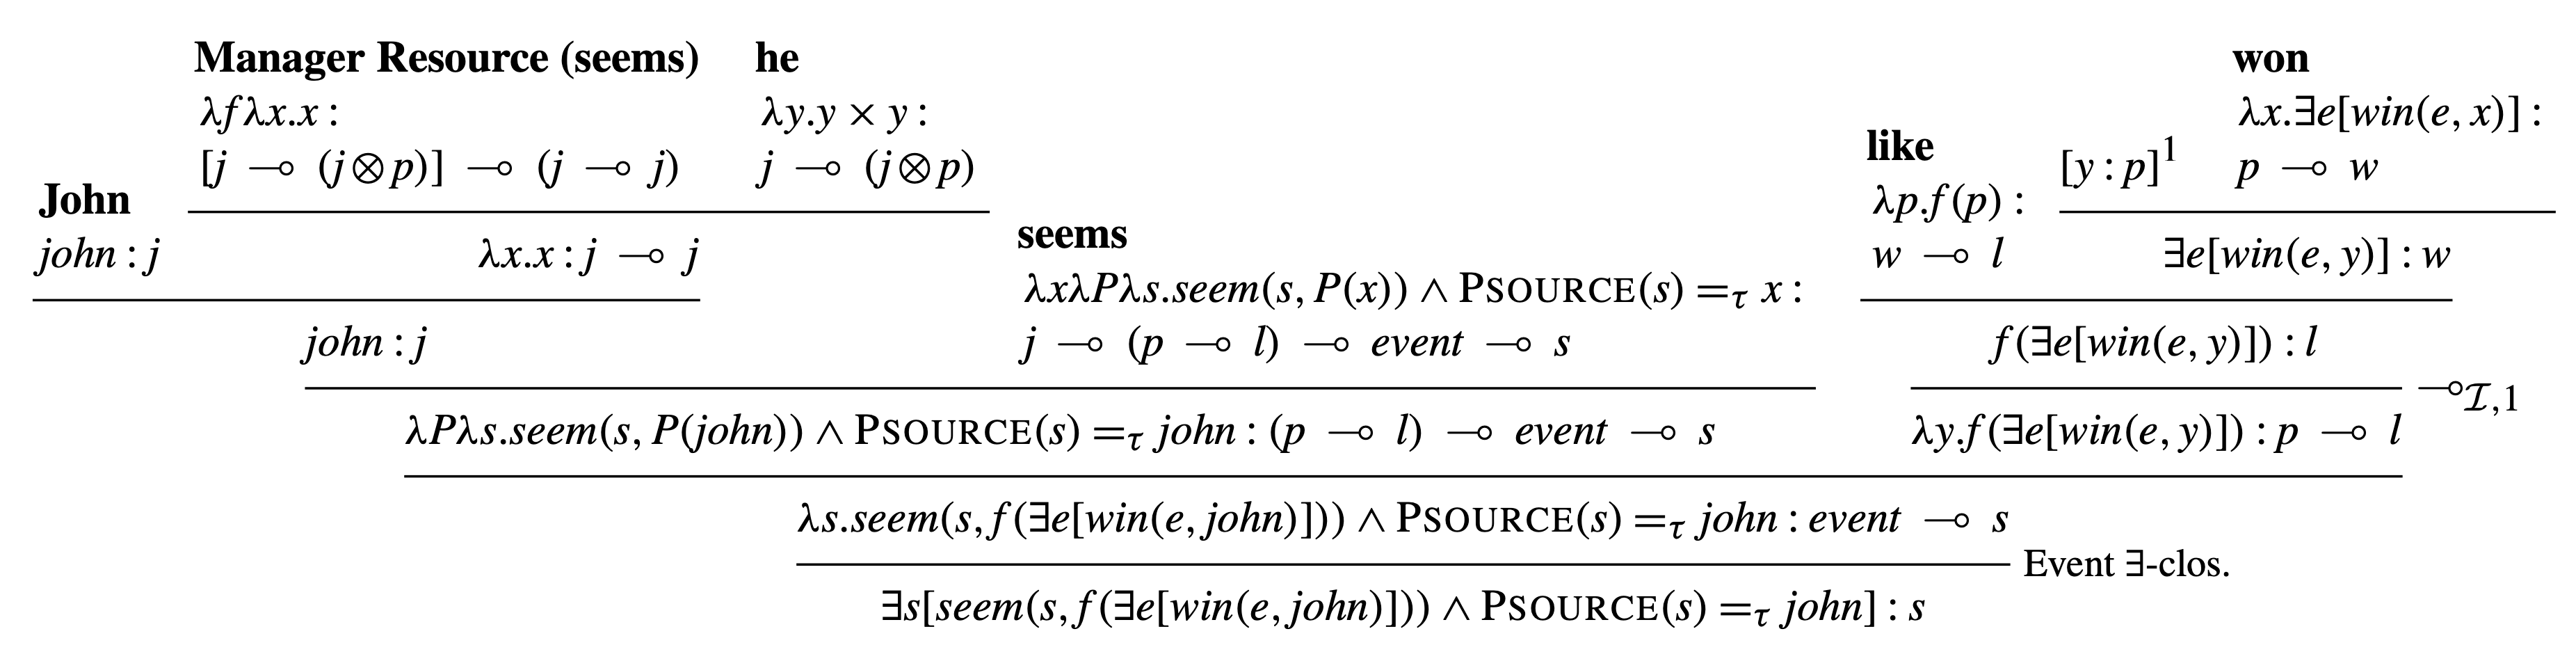
\includegraphics[scale=0.25]{SCR-20240317-bvtm.png}


\begin{itemize}
  \item More complex CR example: matrix subject is coindexed with dative object of ``tell''
\end{itemize}

\ex. \begingl
\gla \textbf{Ti}-dhr-u bħallilieku xi ħadd qal-\textbf{il-kom} biex \textbf{ti}-tilq-u //
\glb \textbf{2}-appear.\textsc{impv-pl} like.that some no.one say.\textsc{pfv.3sgm-\textbf{dat-2pl}} in.what \textbf{2}-leave.\textsc{impv-pl}//
\glft `You appear as if someone told you to leave' //
\endgl

\begin{itemize}
  \item Notice both \avm{\1} and \avm{\2}: \begin{itemize}
      \item There is \textbf{no syntactic representation of \avm{\1} = \avm{\2}}
      \item \avm{\2} is a ``red herring'' for us now, as it's not involved at all in CR: it's just the coindexation between subject of \textit{leave} and dative object of \textit{tell} (regular raising to object, fully independent of CR upstairs)
      \item \avm{\1} represents  syntactic coindexation between matrix subject and the subject of `like'
      \item Importantly, the coindexation between \avm{\1} and the pronominal dative clitic is done semantically, not represented in the syntax
    \end{itemize}
\end{itemize}

\ex. \avm{[
    pred & `\emph{tidhru} <xcomp>\textsc{subj}' \\
    subj & \1 [
      pred & `\textsc{pro}' \\
      pres & 2 \\
      num & \textsc{pl}
    ] \\
    xcomp & [
      pred & `\emph{bħal} <subj, comp>' \\
      subj & \1 \\
      comp & [
        compform & `\emph{likieku}' \\
        pred & `\emph{qal} <subj, obj\(_{\theta}\), xcomp>' \\
        subj & [
          pred & `\emph{ħadd}' \\
          spec  [
            pred & `\emph{xi}'
          ]
        ] \\
        obj\(_{\theta}\) & \2 [
          pred & `\textsc{pro}' \\
          pers & 2 \\
          num & \textsc{pl} \\
          case & \textsc{dat}
        ] \\
        xcomp & [
          compform & `\emph{biex}' \\
          pred & `\emph{titilqu} <subj>' \\
          subj & \2
        ]
      ]
    ]
]}










\section{Comparison}
\begin{itemize}
  \item How do you get Copy-Raising into the grammar? \begin{itemize}
      \item HPSG: a lexical rule creates CR constructions: it converts a subtype of perception verb into a CR verb
      \item LFG: the `like'-element ensures that the same lexical entry for the predicate works for both raising and copy raising configurations
    \end{itemize}

  \item Coindexation 
    \begin{itemize}
      \item HPSG (syntactic): via conindexation of the subject of CR verb with the pronoun, which is also the external argument of the complement clause.
      \item LFG (semantic): while coindexation of the subject of the CR verb with the subject of the complement clause is also present, the coindexation between the pronoun, crucially not the subject of the embedded clause, and the matrix subject is established via a semantic mechanism conceptually similar to null operator movement/lambda abstraction.
    \end{itemize}


  \item Any different predictions?? What should happen in other languages?? 
    \begin{itemize}
      \item  What kind of verbs can end up as CR verbs? 
        \begin{itemize}
          \item HPSG: only a subtype of perception verbs, they don't strictly speaking need to be raising verbs to begin with \begin{itemize}
              \item \textit{sound:} \ding{51} CR (\textit{John sounds like he's happy}), \ding{55} raising (*\textit{John sounds to be happy}; although what about \textit{John sounds happy}?)
            \end{itemize}

          \item LFG: CR, general perception-resemblance, and raising verbs, they all contain a raising configuration
          \item LFG makes the prediction that any raising verb is also a copy raising verb, and vice versa, due to the identical format of the lexical entries of the verb involved in raising and copy raising.
          \item HPSG, on the other hand, says nothing about whether the class of verbs undergoing raising and copy raising are the same or not.
        \end{itemize}

      \item What argument of the embedded clause can be coindexed with the matrix subject? \begin{itemize}
          \item LFG: any argument
          \item HPSG: only the embedded subject; the other cases are not true CR \begin{itemize}
              \item Because coindexation is done with \textsc{xarg}, it can only be very local, not across multiple levels of embedding
              \item If you were dealing with an unbounded dependency (similar to Ā-ones in terms of locality) then you'd need \textsc{gap} feature, not something like \textsc{xarg}
                \ex. Mary seems like some one told John that Bill wants to upset her.

            \end{itemize}
        \end{itemize}
    \end{itemize}
\end{itemize}

\end{document}



